\documentclass[tikz,border=14pt]{standalone}
\usetikzlibrary{positioning,shapes.geometric,fit,shapes,arrows.meta,calc,backgrounds}
\usepackage{amsmath}

\begin{document}
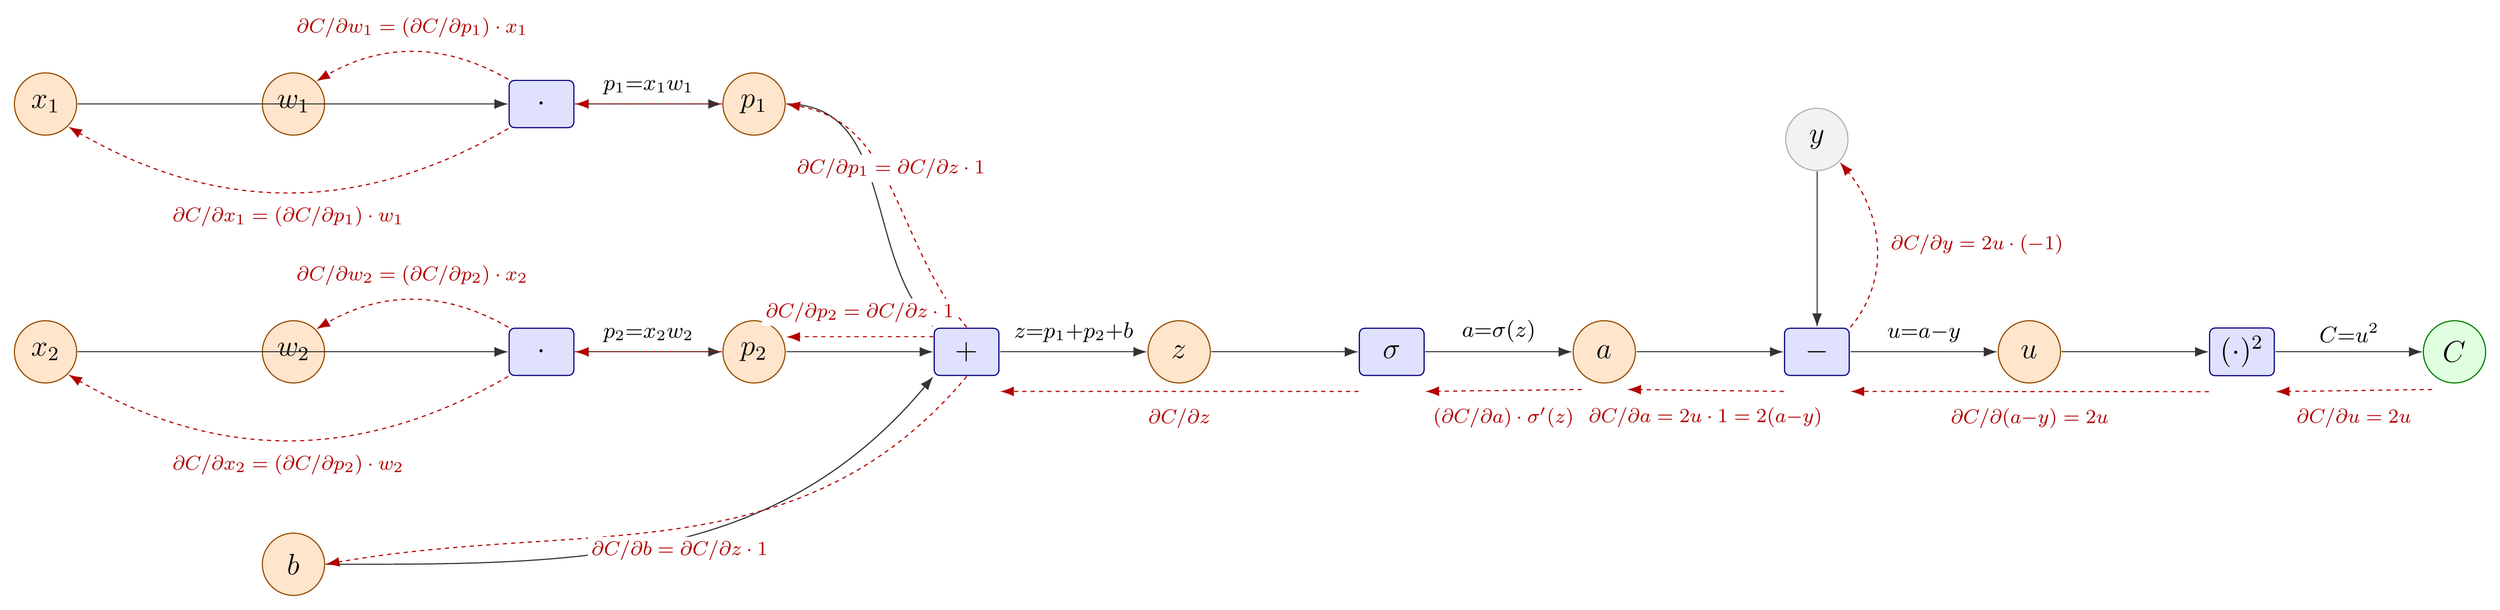
\begin{tikzpicture}[
    scale=1.8, transform shape,
    >=LaTeX,
    % Entradas y parámetros: círculos naranja
    var/.style={
        circle,
        minimum width=2.5em,
        draw=orange!60!black,
        fill=orange!20,
        thick,
        font=\large
    },
    % Operaciones: rectángulos redondeados azul
    op/.style={
        rectangle,
        rounded corners=4pt,
        minimum width=2.6em,
        minimum height=1.9em,
        draw=blue!50!black,
        fill=blue!12,
        thick,
        font=\large
    },
    % Salida / costo: círculo verde
    res/.style={
        circle,
        minimum width=2.5em,
        draw=green!50!black,
        fill=green!12,
        thick,
        font=\large
    },
    % Etiqueta verdadera: círculo gris
    target/.style={
        circle,
        minimum width=2.5em,
        draw=gray!60,
        fill=gray!10,
        thick,
        font=\large
    },
    arrow/.style={-{Latex[length=3.5mm, width=2.5mm]}, thick, black!80},
    backprop/.style={-{Latex[length=3.5mm, width=2.5mm]}, dashed, red!70!black, thick},
    bplabel/.style={font=\footnotesize, text=red!70!black, fill=white,
                    inner sep=1.5pt, rounded corners=1pt},
    fwlabel/.style={font=\small, black}
]

% ══════════════════════════════════════════════════════════════════════════════
% NODOS — espaciado amplio para claridad
% ══════════════════════════════════════════════════════════════════════════════

% --- Rama superior: x₁, w₁ → (·) → p₁ ---
\node[var] (x1)   at (0,    3.5)  {$x_1$};
\node[var] (w1)   at (3.5,  3.5)  {$w_1$};
\node[op]  (mul1) at (7.0,  3.5)  {$\cdot$};
\node[var] (p1)   at (10.0, 3.5)  {$p_1$};

% --- Rama inferior: x₂, w₂ → (·) → p₂ ---
\node[var] (x2)   at (0,    0)    {$x_2$};
\node[var] (w2)   at (3.5,  0)    {$w_2$};
\node[op]  (mul2) at (7.0,  0)    {$\cdot$};
\node[var] (p2)   at (10.0, 0)    {$p_2$};

% --- Flujo central: + → z → σ → a → − → u → (·)² → C ---
\node[op]  (add)  at (13.0, 0)    {$+$};
\node[var] (z)    at (16.0, 0)    {$z$};
\node[op]  (sig)  at (19.0, 0)    {$\sigma$};
\node[var] (a)    at (22.0, 0)    {$a$};
\node[op]  (sub)  at (25.0, 0)    {$-$};
\node[var] (u)    at (28.0, 0)    {$u$};
\node[op]  (sq)   at (31.0, 0)    {$(\cdot)^2$};
\node[res] (C)    at (34.0, 0)    {$C$};

% --- Fila inferior: b ---
\node[var] (b)    at (3.5, -3.0)  {$b$};

% --- Etiqueta verdadera ---
\node[target] (y) at (25.0, 3.0)  {$y$};

% ══════════════════════════════════════════════════════════════════════════════
% FORWARD PASS — flechas sólidas
% ══════════════════════════════════════════════════════════════════════════════

% Entradas y pesos → multiplicaciones
\draw[arrow] (x1.east) -- (mul1.west);
\draw[arrow] (w1.east) -- (mul1.west);
\draw[arrow] (x2.east) -- (mul2.west);
\draw[arrow] (w2.east) -- (mul2.west);

% Multiplicaciones → productos intermedios
\draw[arrow] (mul1.east) -- (p1.west)
    node[midway, above, fwlabel] {$p_1{=}x_1 w_1$};
\draw[arrow] (mul2.east) -- (p2.west)
    node[midway, above, fwlabel] {$p_2{=}x_2 w_2$};

% Productos intermedios + b → suma
\draw[arrow] (p1.east) to[out=0, in=130]
    (add.north west);
\draw[arrow] (p2.east) -- (add.west);
\draw[arrow] (b.east) to[out=0, in=-130]
    (add.south west);

% Suma → z → sigmoide → a
\draw[arrow] (add.east) -- (z.west)
    node[midway, above, fwlabel] {$z{=}p_1{+}p_2{+}b$};
\draw[arrow] (z.east) -- (sig.west);
\draw[arrow] (sig.east) -- (a.west)
    node[midway, above, fwlabel] {$a{=}\sigma(z)$};

% a → resta ← y
\draw[arrow] (a.east) -- (sub.west);
\draw[arrow] (y.south) -- (sub.north);

% resta → u → (·)² → C
\draw[arrow] (sub.east) -- (u.west)
    node[midway, above, fwlabel] {$u{=}a{-}y$};
\draw[arrow] (u.east) -- (sq.west);
\draw[arrow] (sq.east) -- (C.west)
    node[midway, above, fwlabel] {$C{=}u^2$};

% ══════════════════════════════════════════════════════════════════════════════
% BACKPROPAGATION — flechas rojas discontinuas con curvas suaves
% ══════════════════════════════════════════════════════════════════════════════

% [1] C → (·)²  :  ∂C/∂u = 2u
\draw[backprop] ([yshift=-6pt]C.south west) -- ([yshift=-6pt]sq.south east)
    node[midway, below=5pt, bplabel]
    {$\partial C / \partial u = 2u$};

% [2] (·)² → −  :  gradient passes through u
\draw[backprop] ([yshift=-6pt]sq.south west) -- ([yshift=-6pt]sub.south east)
    node[midway, below=5pt, bplabel]
    {$\partial C / \partial(a{-}y) = 2u$};

% [3] − → a  :  ∂u/∂a = 1
\draw[backprop] ([yshift=-6pt]sub.south west) -- ([yshift=-6pt]a.south east)
    node[midway, below=5pt, bplabel]
    {$\partial C / \partial a = 2u \cdot 1 = 2(a{-}y)$};

% [4] − → y  :  ∂u/∂y = −1
\draw[backprop] (sub.north east) to[out=50, in=-50]
    node[bplabel, right=4pt, pos=0.5]
    {$\partial C / \partial y = 2u \cdot(-1)$}
    (y.south east);

% [5] a → σ  :  ∂C/∂z = (∂C/∂a) · σ'(z)
\draw[backprop] ([yshift=-6pt]a.south west) -- ([yshift=-6pt]sig.south east)
    node[midway, below=5pt, bplabel]
    {$(\partial C / \partial a)\cdot\sigma'(z)$};

% [6] σ → z → +  :  gradient passes through z
\draw[backprop] ([yshift=-6pt]sig.south west) -- ([yshift=-6pt]add.south east)
    node[midway, below=5pt, bplabel]
    {$\partial C / \partial z$};

% [7] + → p₁ (curva subiendo)
\draw[backprop] (add.north) to[out=130, in=-10]
    node[bplabel, above=3pt, pos=0.5]
    {$\partial C / \partial p_1 = \partial C / \partial z \cdot 1$}
    (p1.east);

% [8] + → p₂ (directo por arriba)
\draw[backprop] ([yshift=6pt]add.west) -- ([yshift=6pt]p2.east)
    node[midway, above=4pt, bplabel]
    {$\partial C / \partial p_2 = \partial C / \partial z \cdot 1$};

% [9] + → b (curva bajando)
\draw[backprop] (add.south) to[out=-130, in=10]
    node[bplabel, below=3pt, pos=0.5]
    {$\partial C / \partial b = \partial C / \partial z \cdot 1$}
    (b.east);

% [10] p₁ → (·)₁  :  gradient passes through
\draw[backprop] (p1.west) -- (mul1.east);

% [11] (·)₁ → w₁ (curva suave por arriba)
\draw[backprop] (mul1.north west) to[out=150, in=30]
    node[bplabel, above=4pt, pos=0.5]
    {$\partial C / \partial w_1 = (\partial C / \partial p_1)\cdot x_1$}
    (w1.north east);

% [12] (·)₁ → x₁ (curva suave por abajo)
\draw[backprop] (mul1.south west) to[out=-150, in=-30]
    node[bplabel, below=4pt, pos=0.5]
    {$\partial C / \partial x_1 = (\partial C / \partial p_1)\cdot w_1$}
    (x1.south east);

% [13] p₂ → (·)₂  :  gradient passes through
\draw[backprop] (p2.west) -- (mul2.east);

% [14] (·)₂ → w₂ (curva suave por arriba)
\draw[backprop] (mul2.north west) to[out=150, in=30]
    node[bplabel, above=4pt, pos=0.5]
    {$\partial C / \partial w_2 = (\partial C / \partial p_2)\cdot x_2$}
    (w2.north east);

% [15] (·)₂ → x₂ (curva suave por abajo)
\draw[backprop] (mul2.south west) to[out=-150, in=-30]
    node[bplabel, below=4pt, pos=0.5]
    {$\partial C / \partial x_2 = (\partial C / \partial p_2)\cdot w_2$}
    (x2.south east);

\end{tikzpicture}
\end{document}
